\section{4.4}
\subsection{(a)}

Let L1 be the position in code right after the call of f, L2 the position right after the call of doVec, and L3 the position right after our call of sum.
Let @f be the address of procedure f.

\stackenv{
    \stackframe{main}{
        \stackrow{?}{Arbitrary static link for main}
        \stackrow{@main}{Procedure adress}
        \stackrow{?}{Arbitrary return adress for main}
        \stackrow{?}{Arbitrary dynamic link for main}
        \addtocounter{stkctr}{36}
        \stackrow{Values of a}{Local array a}
        \stackrow{Value of i}{Local integer i in main}
    }
    \stackframe{sum}{
        \stackrow{b - 52}{Argument v}
        \stackrow{b - 12}{Static link}
        \stackrow{@sum}{Procedure adress}
        \stackrow{L3}{Return adress}
        \stackrow{b - 12}{Dynamic link}
        \stackrow{Value of s}{Local integer s}
    }
    \stackframe{doVec}{
        \stackrow{b - 52}{Argument v}
        \stackrow{@add}{Address of argument add}
        \stackrow{b - 76}{Static link of argument add}
        \stackrow{b - 12}{Static link}
        \stackrow{@doVec}{Procedure adress}
        \stackrow{L2}{Return adress}
        \stackrow{b - 76}{Dynamic link}
        \stackrow{Value of i}{Local integer i in doVec}
    }
    \stackframe{add}{
        \stackrow{v[i]}{Argument}
        \stackrow{b - 76}{Static link}
        \stackrow{@add}{Procedure adress}
        \stackrow{L1}{Return adress}
        \stackrow{b - 108}{Dynamic link}
    }
}

\textcolor{blue}{Blue} arrows represent static links, \textcolor{red}{red} ones represent dynamic links.

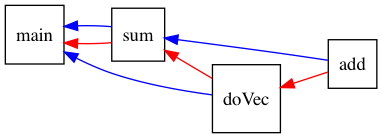
\includegraphics[width=\linewidth]{ex4.png}

\subsection{(b)}
\subsubsection{(i)}
Note that at this point we have the stack from (a) up to \texttt{b - 112}, and that the frame pointer is currently \texttt{b - 108}.
\asmenv{
    \asmr{LDLW 24}{Get v}
    \asmr{LDLW -4}{Get i}
    \asmr{OFFSET}{Get address of v[i]}
    \asmr{LOADW}{Get v[i]}
    \asmr{LDLW 16}{Get static link of f}
    \asmr{LDLW 20}{Get address of f}
    \asmr{PCALLW 1}{Call f}
}

\subsection{(ii)}
Note that at this point we have the entire stack from (a), and the frame pointer is currently \texttt{b - 132}.
\asmenv{
    \asmr{LDLW 12}{Follow static link once}
    \asmr{LDNW -4}{Get s}
    \asmr{LDLW 16}{Get x}
    \asmr{BINOP PLUS}{Calculate s + x}
    \asmr{LDLW 12}{Follow static link once}
    \asmr{STNW -4}{Set s to s + x}
}

\subsubsection{(iii)}
Note that at this point we have the stack from (a) up to \texttt{b - 80}, and that the frame pointer is currently \texttt{b - 76}.
\asmenv{
    \asmr{LDLW 16}{Get v}
    \asmr{GLOBAL \_add}{Get address of procedure add}
    \asmr{LOCAL 0}{Get static link for procedure add}
    \asmr{LOCAL 0}{Get static link}
    \asmr{PCALLW 3}{Call procedure with 3 arguments (closure counts as 2)}
}

\subsection{(c)}
In this case, several things would need to change:
\begin{itemize}

\item We must arrange for \texttt{v} to be copied to the stack as an argument when calling \texttt{sum} or \texttt{doVec}.
\item We must arrange for \texttt{v} to be properly aligned to word boundaries.
\item When calling these functions, the number of words used for arguments must take into account the lengths of \texttt{v}, and its alignment.
\item When using local variables in these functions, we must take into account the lengths and alignements of arrays when accessing parameters held deeper in the stack than them.
\item When using elements in these vectors, we must use one less indirection.

\end{itemize}

One case when it might be faster to copy the entire array is when dealing with small arrays placed in distant spots in memory, that are used very many times. In such cases, the importance of locality of reference dominates, and the one time cost of copying the arrays is insignificant. If our language has only unaliased arrays, like PicoPascal or Fortran, we can introduce an optimisation that makes code that passes by reference just as fast:
\begin{itemize}
\item Identify often used, small arrays.
\item Start simulating the array with registers once we reach an area when the array is often used.
\item Upon exiting this area, write the values in the registers to the array.
\end{itemize}
